\chapter{Forståelsesgrundlag}
\section{Analog-to-digital converter}
I dette afsnit beskrives hvordan ADC'en er opsat. Der fokuseres på de parametre der har været ændret og tilpasset i forhold til dette projekt.

\begin{figure}[H]
	\centering
	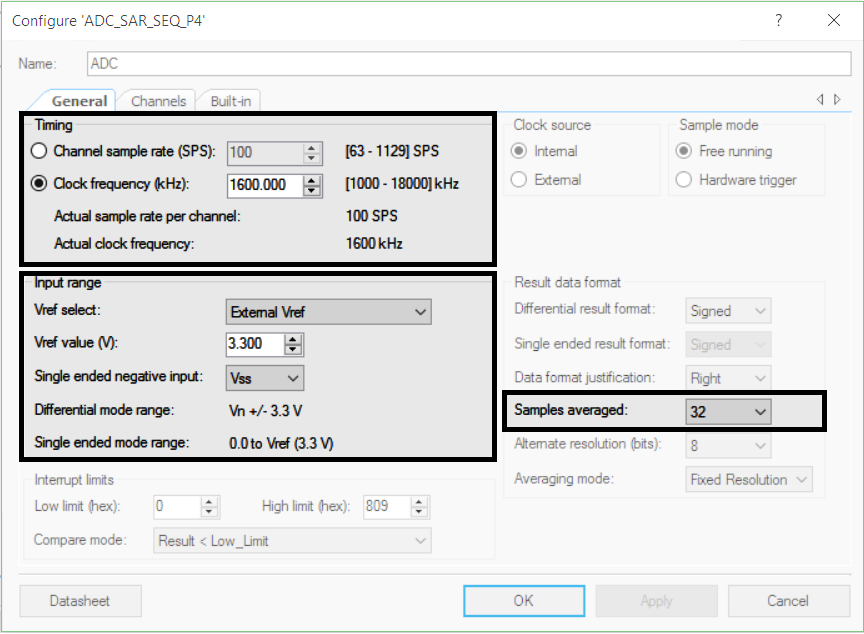
\includegraphics[width=0.5\textwidth]{fig/ADC_instillinger_edit.png}
	\caption{Heraf fremgår ADC's generelle indstillinger, hvor de fremhævede områder viser parametre relevant for dette projekt. Øverste blok til venstre viser instillingsmuligheder for samplingsfrekvens samt clock frekvens, samt de aktuelle frekvenser. Nederste blok til venstre viser instillinger for ADC'ens arbejdsområde i forhold til single ended og differential måling. Blokken til højere viser mængden af samples fortaget til at give en gennemsnitlig sample.}
	\label{fig:ADC_GeneralTab}
\end{figure}

\textbf{Bestemmelse af samplingsfrekvens:}
Område 1 af \autoref{fig:ADC_GeneralTab}, viser indstillingerne for ADC'en samplingsfrekvens, samt clock frekvens. Ved indstilling af disse frekvenser udregnes en reel sampling- og clock frekvens der oplyses nedenfor. De reelle frekvenser kan variere grundet andre parametre som antal af kanaler, konverteringstid, mm. Yderligere parametre kan findes i databladet for ADC'en. 

\noindent
I dette projekt er en samplingsfrekvens på $100~Hz$ opnået ved at definere en clockfrekvens på $1600~kHz$ samt justering for konverteringstiden af kanalerne der ses i \autoref{fig:ADC_KanalTab}. Hertil er der pålagt en forsinkelse således en konverteringstid på $3,32~ms$ per kanal opnås. Dette giver en konverteringstid på $9,96~ms$ for de 3 kanaler, hvilket ADC'en oplyser som en aktuel samplingsfrekvens på $100~Hz$. 

\begin{figure}[H]
	\centering 
	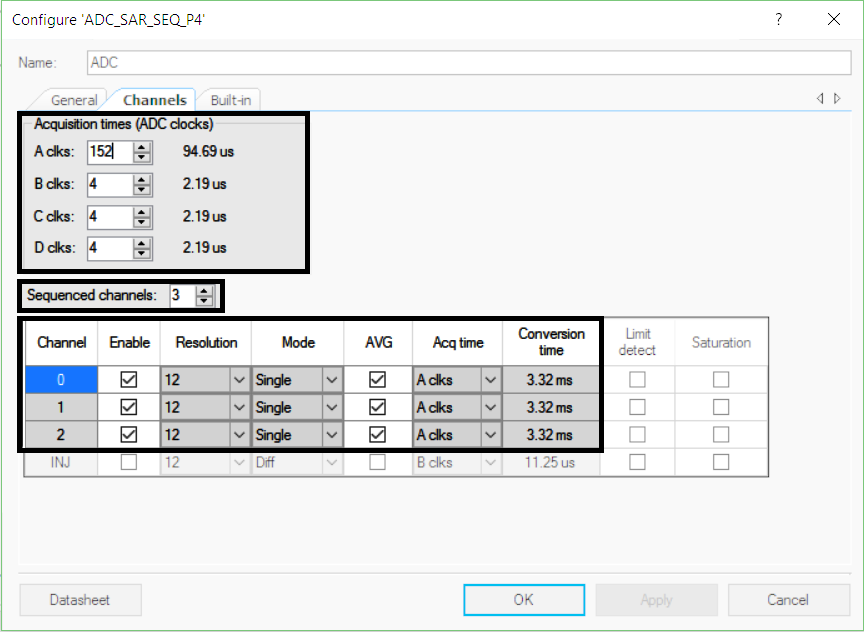
\includegraphics[width=0.5\textwidth]{fig/ADC_instillinger2_edit.png}
	\caption{Indstillinger for at input til ADC. Øverste blok viser indstillingsmuligheder for 4 ADC clocks, der definere konverteringstiden for kanalerne. Miderste blok viser antallet af kanaler der defineres. Nederste blok viser indstillingsmuligheder, samt konvertieringstid for de enkelte kanaler.}
	\label{fig:ADC_KanalTab}
\end{figure}

\textbf{Arbejdsområde for ADC:}
Område nummer 2 af \autoref{fig:ADC_GeneralTab}, viser indstillingerne for ADC'ens arbejdsområde. Vref definere størrelsen af arbejdsområdet, hvortil en ekstern reference er valgt. Denne reference sættes identisk med mikrokontrollerens forsyning til acceleromterne på $3,3~V$. Det negative input for single ended målinger sættes til Vss (jord). Dette giver et arbejdsområde for single ended målinger på $0,0~V - 3,3~V$. Da det negative input tilsluttes jord, falder opløsningen $1~bit$, da der ikke kan forekomme negative udslag i arbejdsområdet. 

\textbf{Gennemsnits samples:}
Område 3 af \autoref{fig:ADC_GeneralTab} er indstillingen for hvor mange samples der anvendes for hver af kanalerne til at repræsentere én konverteret sample. Heraf benyttes 32 samples til at udregne en gennemsnits sample. Dette gøres kun gældende for kanaler hvor 'AVG' er tilvalgt, som det ses af nederste blok i \autoref{fig:ADC_KanalTab}. Dette er implementeret da samplingsfrekvens på $100~Hz$ stadig opretholdes, samt at v 





